\documentclass[12 pt]{article}
\usepackage[margin = 1cm]{geometry}
\usepackage [utf8]{inputenc}
\usepackage[T2A]{fontenc}
\usepackage[russian]{babel}
\usepackage{amsthm, amsmath, amssymb}
\usepackage{xcolor}
\definecolor{mygreen}{rgb}{0,0.6,0}
\usepackage{listings}
\usepackage{graphicx}
\lstset{
  language=Java,
  tabsize=2,
  belowcaptionskip=1\baselineskip,
  breaklines=true,
  xleftmargin=1cm,
  escapechar=|,
  showstringspaces=false,
  commentstyle=\color{green},
  keywordstyle=\color{blue},
  stringstyle=\color{mygreen},
  basicstyle=\footnotesize\ttfamily,
  numbers=left,
  commentstyle=\usefont{T2A}{fcr}{m}{sl}
}

\renewcommand{\O}{\mathcal{O}}
\newcommand{\SO}{\Rightarrow}
\newcommand{\EQ}{\Leftrightarrow}
\newcommand{\union}{\cup}
\renewcommand{\div}{\mathop{\raisebox{-2pt}{\vdots}}}

\begin{document}

\section{Android Manifest}
    \begin{itemize}
    	\item Описание проекта, в том числе настройки и конфигурация.
    	\item Прописаны permission и составляющие проекта, такие как:
		\begin{enumerate}
        	\item Activity 
        	\item BroadCastReceiver 
        	\item Service
        \end{enumerate}
    \end{itemize}

\section{Activity}
    \begin{itemize}
    	\item Экран приложения
        \item Первой в программе вызывается Activity, к которому приходит интент MAIN. Это также прописывается в Android Manifest.
    	\item Цикл жизни:
   	\end{itemize}
	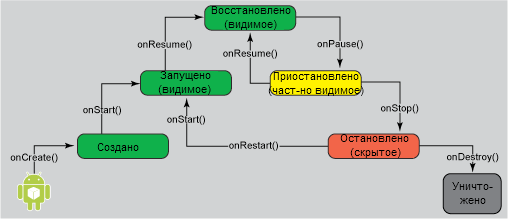
\includegraphics{LifeCycle.png}
    
\section{BroadCastReceiver} 
    
    BroadCastReceiver - класс-обработчик широковещательных сообщений(intent). Может быть подписан на несколько разных интентов. Если к нему приходит несколько интентов за раз, то они выстраиваются в цепочку и обрабатываются по одному, поэтому интент не обрабатывается дольше 5 секунд, чтобы другие не ждали. Из-за этого количество действий, которое вы можете сделать с помощью BroadCastReceiver, довольно ограничено(обычное использование - послать другой интент, чтобы запустить Activity, Service или что-нибудь подобное).
    
    Другое назначение BroadCastReceiver это получать системные оповещения, такие как оповещения о маленьком заряде батарейки или о том, что Android загрузился.
    
    BroadCastReceiver региструется в Android Manifest'е так:
    \begin{lstlisting}
<receiver android:name=".LocationChangedReceiver" />
    \end{lstlisting} 
    
    В принципе, можно регистрировать и программно.
    
    Указать, на какие intent'ы подписан BroadCastReceiver, можно двумя способами:
	\begin{itemize}
    	\item В Android Manifest (обычно при подписке на системные события)
		\item Программно:
        \begin{lstlisting}
mLocationManager = (LocationManager)getSystemService(Context.LOCATION_SERVICE);
Intent intent = new Intent(this, LocationChangedReceiver.class);
mLocationChangedIntent =
PendingIntent.getBroadcast(this, 0, intent, PendingIntent.FLAG_UPDATE_CURRENT);
    \end{lstlisting}
    \end{itemize}
     Здесь:
	\begin{itemize}
    \item Получаем доступ к LocationManager
	\item Создаем Intent и прописываем класс, куда интент должен быть направлен.
	\item Создаем PendingIntent от нашего Intent.
    \end{itemize}
	Класс Intent - это такой способ общаться между частями приложения. В него можно записать дополнительную информацию.
        \begin{lstlisting}
startService.putExtra(LocationManager.KEY_LOCATION_CHANGED, location);
        \end{lstlisting}        
        
    Доставать информацию из Intent можно так:
        \begin{lstlisting}
Location location = (Location) intent.getExtras().get(locationKey);
        \end{lstlisting}
    PendingIntent - наследник класса Intent. Главное его отличие от обычного интента в том, что он учитывает права приложения. Можно запускать Activity(приложение) из другого приложения, но у этого Activity(приложения) может не быть прав на работу с некоторыми ресурсами. Если эти права нужны, вы можете послать PendingIntent и передать тем самым Activity(приложению), которое вы запускаете, свои права на исполнение. Также некоторые API просто по умолчанию используют PendingIntent(например, так делает LocationManager). 
    
      Интенты бывают:
      \begin{itemize}
      		\item explicit - для них явно прописывается, к какому классу его отправить
            \item implicit - неявно описывается, куда нужно передать сообщение. Дальше в этом разбирается Android.
      \end{itemize}
      В коде выше интент - explicit. 
    
    Когда приходит интент, который предназначен для данного BroadCastReceiver, вызывается метод onReceive(). Одним из его аргументов является экземпляр класса Context - базовый класс для частей приложения. Через него можно обращаться к ресурсам системы. К примеру, Activity - наследник класса Context. Поэтому, мы можем вызвать, к примеру, метод getSystemService(), определённый в классе Context - для доступа к какому-то сервису. А вот BroadCastReceiver не является наследником класса Context, но доступ к различным менеджерам может понадобиться, поэтому контекст и передаётся методу onReceive(). 
    
        В нашем Receiver мы просто напечатаем в Log некое сообщение(что такое Log мы поподробнее ещё обсудим). 
        
        \begin{lstlisting}
public class LocationChangedReceiver extends BroadcastReceiver {

    private static final String TAG = LocationChangedReceiver.class.getSimpleName();

    public LocationChangedReceiver() { }

    @Override
    public void onReceive(Context context, Intent intent) {
        final String locationKey = LocationManager.KEY_LOCATION_CHANGED;

        if (intent.hasExtra(locationKey)) {
            Location location = (Location) intent.getExtras().get(locationKey);

            Intent startService = new Intent(context, ForecastUpdateService.class);
            startService.putExtra(LocationManager.KEY_LOCATION_CHANGED, location);
            context.startService(startService);
        }
    }
}
    \end{lstlisting}
    
    Если обобщить:
    \begin{itemize}
        \item Один из стандартных классов Android, завязан на несколько(может один) intent. 
	    \item Получает intent, к которому он привязан и \textcolor{red}{быстро} реагирует(с технической точки зрения при получении intent вызывается onReceive(), который должен быстро выполняться).
		\item Если один BroadCastReceiver соответствует нескольким intent, то они построятся в цепочку и будут выполняться последовательно.
		\item Поэтому если по какому-то intent метод выполняется слишком долго, то его выполнение оборвется, чтобы другие intent не ждали.
		\item Так что обычно, его используют только чтобы послать какой-то другой intent или получить системное оповещение.
 		\item Receiver должен быть прописан в Android Manifest.
        \begin{lstlisting}
<receiver android:name=".LocationChangedReceiver" />
        \end{lstlisting}		    
 	    \item Подписку на intent можно тоже записать в Manifest.
        \item А можно это сделать и програмно. Explicit intent - явно указываем класс, к которому intent отправить. Бывает ещё implicit intent.  
        \item Класс Context - это базовый класс для частей приложения. К примеру, Activity - наследник класса Context. Он предоставляет доступ ко всем андроидовским ресурсам и поэтому является параметром метода onReceive у BroadcastReceiver.
    \end{itemize}

\section{Log}     
    \begin{itemize}
        \item Записи в log выводятся на экран Device Monitor.Logcat.
        \item Логирование происходит так:
    \end{itemize}
    \begin{lstlisting}
    ...
private static final String TAG = 
            SMSReceiver.class.getSimpleName();
    ...
Log.d(TAG, "SMS received");    
    \end{lstlisting}

    \section{Service}    
    \begin{itemize}
        \item Service также надо прописывать в манифесете:
        \begin{lstlisting}
<service
    android:name=".DatabaseService"
    android:exported="false" >
</service>        
        \end{lstlisting}
        \item Для того, чтобы делать продолжительные действия BroadCastReceiver не подходит. Для этого нужно использовать Service.
        \item Ключ exported задаёт, позволено ли другим приложениям запускать наш сервис, Activity и тд.
        \item Если к нему обращаются много intent, они также становятся в очередь.
        \item Запускают intent к service через команду startService(...);
        \item При обработке intent запускается метод onHandleIntent(Intent intent);
    \end{itemize}
    
\section{Permissions}
    \begin{itemize}
        \item Чтобы работать с сетью надо подключить соотетсвующие permission.
        \begin{lstlisting}
<uses-permission android:name="android.permission.INTERNET" /> 
<uses-permission  android:name="android.permission.ACCESS_NETWORK_STATE"/>        
        \end{lstlisting}
    \end{itemize}
    
\section{Connection}
    \begin{itemize}
        \item Самый простой способ работать с сетью - это HttpURLConnection.
        \item Возвращается методом .openConnection():
        \begin{lstlisting}
URL url = new URL(uri.toString());
connection = 
        (HttpURLConnection) url.openConnection();
        \end{lstlisting}
        \item Протокол http может обрабатывать различные запросы. Например, запрос на получение информации. Если мы хотим получить информацию - пишем следующее:
        \begin{lstlisting}
connection.setRequestMethod("GET");
connection.connect();
        \end{lstlisting}
    \end{itemize}
    Пример считывания информации:
    \begin{lstlisting}
InputStream inputStream = connection.getInputStream();
StringBuilder buffer = new StringBuilder();
if (inputStream == null) {
    return;
}
reader = new BufferedReader(new InputStreamReader(inputStream));
String line;
while ((line = reader.readLine()) != null) {
    buffer.append(line);
    buffer.append("\n");
}

if (buffer.length() == 0) {
    return;
}
    \end{lstlisting}
\end{document}